\documentclass[a4paper,11pt]{article}

% Kodovani (cestiny) v dokumentu: utf-8
%\usepackage[cp1250]{inputenc}	% Omezena stredoevropska kodova stranka, pouze MSW.
\usepackage[utf8]{inputenc}	% Doporucujeme pouzivat UTF-8 (unicode).

\usepackage[margin=2cm]{geometry}
\newtoks\jmenopraktika \newtoks\jmeno \newtoks\datum
\newtoks\obor \newtoks\skupina \newtoks\rocnik \newtoks\semestr
\newtoks\cisloulohy \newtoks\jmenoulohy
\newtoks\tlak \newtoks\teplota \newtoks\vlhkost

\jmenopraktika={Fyzikální praktikum 1}
\jmeno={Lukáš Lejdar}
\datum={26. března 2023}
\obor={F}
\skupina={Út 16:00}

\cisloulohy={9}
\jmenoulohy={Měření elektrického napětí a proudu}

\tlak={101{,}35}
\teplota={21,1}
\vlhkost={47,7}


%%%%%%%%%%% Uzitecne balicky:
\usepackage[czech]{babel}
\addto\captionsczech{}

\usepackage{graphicx}
\usepackage{amsmath}
\usepackage{xspace}
\usepackage{url}
\usepackage{indentfirst}
\usepackage{wrapfig}

%%%%%% Zamezeni parchantu:
\widowpenalty 10000 \clubpenalty 10000 \displaywidowpenalty 10000
%%%%%% Parametry pro moznost vsazeni vetsiho poctu obrazku na stranku
\setcounter{topnumber}{3}	  % max. pocet floatu nahore (specifikace t)
\setcounter{bottomnumber}{3}	  % max. pocet floatu dole (specifikace b)
\setcounter{totalnumber}{6}	  % max. pocet floatu na strance celkem
\renewcommand\topfraction{0.9}	  % max podil stranky pro floaty nahore
\renewcommand\bottomfraction{0.9} % max podil stranky pro floaty dole
\renewcommand\textfraction{0.1}	  % min podil stranky, ktery musi obsahovat text
\intextsep=8mm \textfloatsep=8mm  %\intextsep pro ulozeni [h] floatu a \textfloatsep pro [b] or [t]

% Tecky za cisly sekci:
\renewcommand{\thesection}{\arabic{section}.}
\renewcommand{\thesubsection}{\thesection\arabic{subsection}.}
% Jednopismenna mezera mezi cislem a nazvem kapitoly:
\makeatletter \def\@seccntformat#1{\csname the#1\endcsname\hspace{1ex}} \makeatother
%
\newcommand{\vsn}[4]{\ensuremath{#1 =} #2(#3)\,#4}
\newcommand{\vrn}[6]{\ensuremath{#1 =} (#2 $\pm$ #3)\,#4 ($p=$ #5\,\%, $\nu=$ #6)}


%%%%%%%%%%%%%%%%%%%%%%%%%%%%%%%%%%%%%%%%%%%%%%%%%%%%%%%%%%%%%%%%%%%%%%%%%%%%%%%
% Zacatek dokumentu
%%%%%%%%%%%%%%%%%%%%%%%%%%%%%%%%%%%%%%%%%%%%%%%%%%%%%%%%%%%%%%%%%%%%%%%%%%%%%%%

\begin{document}

\thispagestyle{empty}

{
\begin{center}
\sf 
{\Large Ústav fyziky a technologií plazmatu Přírodovědecké fakulty Masarykovy univerzity} \\
\bigskip
{\huge \bfseries FYZIKÁLNÍ PRAKTIKUM} \\
\bigskip
{\Large \the\jmenopraktika}
\end{center}

\bigskip

\sf
\noindent
\setlength{\arrayrulewidth}{1pt}
\begin{tabular*}{\textwidth}{@{\extracolsep{\fill}} l l}
\large {\bfseries Zpracoval:}  \the\jmeno & \large  {\bfseries Naměřeno:} \the\datum\\[2mm]
\large  {\bfseries Obor:} \the\obor  \hspace{40mm}  {\bfseries Skupina:} \the\skupina %
&\large {\bfseries Testováno:}\\
\\
\hline
\end{tabular*}
}

\bigskip

{
\sf
\noindent \begin{tabular}{p{4cm} p{0.6\textwidth}}
\Large  Úloha č. {\bfseries \the\cisloulohy:} \par
\smallskip
$T=\the\teplota$~$^\circ$C \par
$p=\the\tlak$~kPa \par
$\varphi=\the\vlhkost$~\%
&\Large \bfseries \the\jmenoulohy  \\[2mm]
\end{tabular}
}

\vskip1cm

\section{Úvod}

V úloze se budeme zabývat měřením vnitřního odporu ručkového ampérmetru a navržením obvodů pro rozsíření jeho rozsahu.
Druhá část úlohy je zaměřená na digitálně analogové a analogově digitální převodníky a jejich vlastnosti.

\section{Teorie}

\subsection{Měření vnitřního odporu ampérmetru}

Určit vnitřní odpor ručkového ampermetru jde jednoduše přímo z Ohmova zákona zapojením obvodu z obrázku 1.


\begin{figure}[htpb]
  \centering
  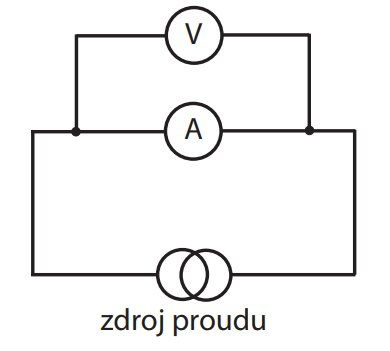
\includegraphics[width=0.3\textwidth]{mereni_voltmetrem.jpg}
  \caption{Měření vnitřního odporu ampérmetru z Ohmova zákona}
\end{figure}

2. možnost využívá nastavitelného odporu podle obrázku 2. 
Nejprve necháme dekádu nepřipojenou a řiditelným zdrojem nastavíme na ampérmetru
maximální výchylku rozsahu $I_0$. Poté dekádu připojíme a snažíme se nastavením hodnoty jejího odporu dosáhnout poloviční výchylky $I = \frac{I_0}{2}$. Nyní protéká oběma větvemi stejný proud, což nastane právě tehdy, když obě větve mají stejný odpor.

\begin{figure}[htpb]
  \centering
  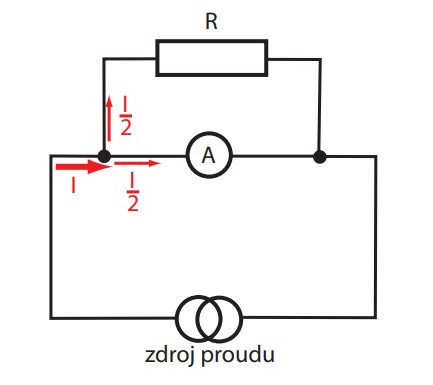
\includegraphics[width=0.35\textwidth]{mereni_dekadou.jpg}
  \caption{Měření vnitřního odporu ampérmetru pomocí odporové dekády}
\end{figure}


\subsection{změna rozsahu ampérmetru}

Obecně můžeme rozsah přístroje pouze zvětšit. Měřený proud jde pomocí bočníku rozdělit do dvou větví a proud se měří jen v jdené, jako na obrázku 3. Celkový proud dopočítáme se znalostí odporu bočníku $R_B$.

\begin{figure}[htpb]
  \centering
  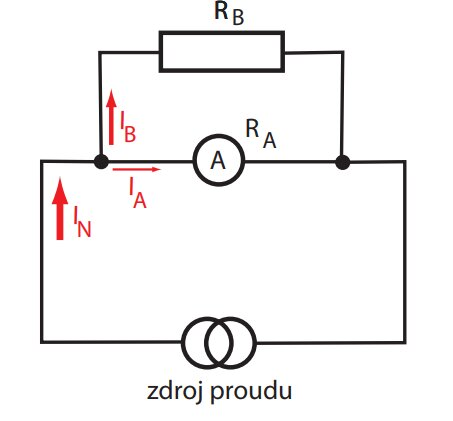
\includegraphics[width=0.35\textwidth]{bocnik.jpg}
  \caption{Zapojení bočníku}
\end{figure}

Protože napětí je na měřicím přístroji i na celkovém obvodu je stejné

\begin{align}
  \frac{I_N}{R_A + R_B} &= R_AI_A = U \\
  R_B &= \frac{R_A}{\frac{I_N}{I_A} - 1},
\end{align}

\noindent
kde $I_N$, je celkový proud a $I_A$ měřený proud ampérmetrem. Vztah (2) udává potřebnou volbou $R_B$ pro $\frac{I_N}{I_A}=$n-násobného zvětšení rozsahu proudu.

\subsection{Změna rozsahu voltmetru}

Namísto paralelně zapojeného bočníku je v případě změny rozsahu voltmetru třeba použít sériově
zapojený odpor, tzv. předřadník (zapojení předřadníku je na obr. 4). 
Místo voltmetru se taky dá použít ampérmetr se známým vnitřním odporem a napětí spočítat z ohmova zákona.

\newpage

\begin{figure}[htpb]
  \centering
  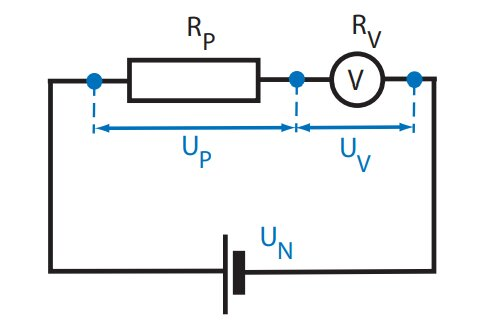
\includegraphics[width=0.4\textwidth]{preradnik.jpg}
  \caption{Zapojení předřadníku}
  \label{fig:}
\end{figure}

Protože proud, který teče voltmetrem je stejný jako ten, který teče celým obvodem,

\begin{align}
  \frac{U_V}{R_V} =& \frac{U_N}{R_P + R_V} \\
  R_P =& (\frac{U_N}{U_V} - 1) R_V, \\ 
\end{align}

\noindent
kde $\frac{U_N}{U_A} = n$, což je keficient zvětšení rozsahu. Pokud namísto voltmetru použijeme ampérmetr,

\begin{align}
  U_N &= (R_A + R_B) * I_A \\
  R_B &= \frac{U_N}{I_A} - R_A.
\end{align}


\subsection{Digitální část}

Číslený rozsah n-bitového převodníku určíme jako $[0, 2^n -1]$ a jeho kvantizační krok 

\begin{align}
  k = \frac{U_m - U_0}{2^n -1},
\end{align}

\noindent
kde $U_0$ je minimální a $U_m$ maximální napětí. Pokud pro žádané napětí hledáme odpovídající vstup použijeme,

\begin{align}
  x = \frac{U(x) - U_0}{k}
\end{align}

Na obrázku 5 je uvedený jeden možný n-bitový přechodník, který obecně patří do skupiny převodníků konstruovaných pro mapování rozsahu (0, $2^n -1$) na napěťový rozsah (0, $U_m$). Reálné získané napětí ale může být odlišné. Zavádíme proto veličny charakterizující tyto odchylky jako

\begin{align}
  \text{chyba ofsetu} & & \delta_0 &= \frac{U_0}{k} & &\\
  \text{chyba zesílení} & & \delta_m &= \frac{U_m - U_0}{k},
\end{align}

\begin{figure}[htpb]
  \centering
  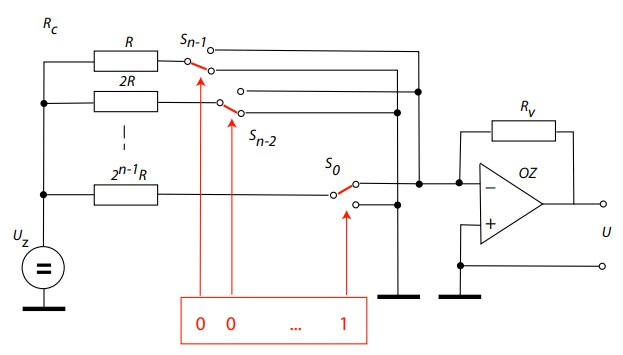
\includegraphics[width=0.8\textwidth]{da_prevodnik.jpg}
  \caption{D/A převodník s váhovými rezistory}
\end{figure}

\newpage

\section{Výsledky měření}

\subsection{Měření vnitřního odporu ampérmetru}

Použili jsme dvě metody měření vnitřního odporu ampérmetru $R_A$. Přímo z ohmova zákona zapojením obvodu z obrázku 1 apomocí odporové dekády podle obrázku 2. 

\begin{table}[htpb]
  \centering
  \begin{tabular}{ c | c }
    měření z Ohmova zákona & 1650(50) $\Omega$ \\
    měření Dekádou & 1670(20) $\Omega$
  \end{tabular}

  \caption{výsledky měření vnitřního odporu ručkového ampérmetru}
\end{table}

\subsection{Zvětšení rozsahu ampérmetru}

N-násobné zvětšení rozsahu můžeme realizovat zapojením obvodu z obrázku 3 s odporem $R_B$, který spočítáme ze 
vztahu (2) se seznalostí $R_A$. Nejjednodušší způsob kontroly je použít velmi přesný 
nastavitelný zdroj napětí a nastavit ho tak, aby na ručkovém ampérmetru byl právě maximální hodnota. 
Nakonec provnáme předpokládanou hodnotu proudu s tou nastavenou na zdroji.

\begin{table}[htpb]
  \centering
  \begin{tabular}{ | c | c | c | c | c | }
    \hline
    n & $R_B$ [$\Omega$] & $I_A$ [$\mu A$] & předpokládáme $I=nI_0$ [mA] & opravdový proud $I$ [mA] \\\hline
    5 & 420(5) & 100 & 0.5 & 0.4929 \\
    10 & 187(2) & 100 & 1 & 0.9790 \\
    20 & 88(1)& 100 & 2 & 1.9664 \\\hline
  \end{tabular}
  \caption{Tabulka měření proudu použitím bočníku podle vztahu (2)}
\end{table}

\subsection{Zvětšení rozsahu voltmertu}

Se znalostí vnitřního odporu jde ampérmetr použít jako voltmetr. S přeřadníkem s odporem $R_P$ podle obvodu z obrázku 4 můžeme navíc zvětšit jeho rozsah na hodnotu $U_N$ podle vztahu (7).
Ke kontrole použijeme podobný postup jako u bočníku.


\begin{table}[htpb]
  \centering
  \begin{tabular}{| c | c | c | c | c | }
    \hline
    předpokládané napětí $U_N$ $[V]$ & $I_A$ [$\mu A$] & $R_B$ [$k\Omega$] & opravdové napětí $U_N$ [V] \\\hline
    5 & 100 & 48.320 & 5.086 \\
    10 & 100 & 98.320 & 10.420 \\\hline
  \end{tabular}
  \caption{Tabulka měření napětí použitím přeřadníku podle vztahu (7)}
\end{table}


\subsection{D/A převodníky}

Určíme rozsah 8-bitového převodníku MDAC08 a 16-bitobého USB - 9162.

\begin{table}[htpb]
  \centering
  \begin{tabular}{ | c | c | c | c | c | }
    \hline
    převodník & n & $U_m$ [V] & $U_0$ [V] & k \\\hline
    MDAC08 & 8 & 9.88121 & $1.2560 * 10^{-3}$ & $38.6 * 10 ^ {-3} $  \\
    USB - 9162 & 16 & 10.6970 & -10.6735 & $0.326 * 10 ^ {-3} $ \\\hline
  \end{tabular}
  \caption{rozsahy dvou D/A převodníků a jejich kvantizační kroky}
\end{table}

Interpolací teď můžeme podle vztahu (9) nastavit libovolné napětí v rozsahu. Třeba pro $U(x) = 3.2$ je x = 42545. 
Skutečné napětí bylo $3.19917$ V. \\

Nominální rozsah přvodníku MDAC08 je 0 - 10 V. Ze vztaů (10) a (11) můžeme určit chybu ofsetu a chybu zesílení jako

\begin{align}
  \delta_0 &= 1.26 * 10^{-3}\\
  \delta_m &= 11.8 * 10^{-3}.
\end{align}

\subsection{Vliv vzorkovací frekvence na kvalitu záznamu}

Zaznamenávali jsme signál o frekvenci 1kHz A/D převodníkem a růžnými vzorkovacími frekvencemi. Výsledky jsou uvedeny v tabulce 3.

\begin{table}[htpb]
  \centering
  \begin{tabular}{ | c | c | }
    \hline
    Vzorkovací frekvence & frekvence záznamu \\\hline
    20 kHz & 1 kHz \\
    2 kHz & 1 kHz \\
    1,1 kHz & 100 Hz \\
    1 kHz & - \\
    100 Hz & - \\\hline
  \end{tabular}
  \caption{Vliv vzorkovací frekvence na kvalitu záznamu A/D převodníku}
\end{table}

\subsection{Kvantizační krok A/D převodníku}

Kvantizační krok vyjadřuje minimální rozdíl napětí, který jde A/D převodníkem změřit. 
K jeho určení existuje následující postup; Zkratováním vstupních svorek začne karta měřit malé náhodné rozdíly napětí. Kvantizační krok se v získaných datech, projeví jako nejmenší nenulový rozdíl dvou následujících hodnot. Použili jsme 12-bitový A/D převodník na kartě ICP DAS PCI-1202LU z měřícího systému ISES. Nejmenší naměřený rozdíl byl 1.22099 mV.

\newpage

\section{Závěr}

Použil jsem dvě různé metody pro měření vnitřního odporu ručkového ampérmetru. Obě měření uvedené v tabulce 1 jsou docela přesné a zhodují se. Dál jsme chtěli zvětšit měřící rozsah. Podle vztahů (2) a (7) jsem odhadl velikosti odporů bočníků a přeřadníků a výsledky uvedl v tabulkách 2 a 3. Rozdíl vypočítaných hodnot a skutečných byl v obou případech minimální. \\

Určil jsem velikosti kvantizačních kroků dvou D/A přeřadníků MDAC08 a USB - 9162 uvedné v tabulce 4. Povedlo se správně odhadnout potřebné vstupní číslo pro nastavení 3.2 V a chyby ofsetu a zesílení byli obě minimální. \\

V tabluce 5 jsme testovali různé vzorkovací frekvence pro měření signálu o frekvenci 1 kHz. Ke spolehlivým výsledkům bylo potřeba alespoň dvojnásobná vzorkovací frekvence. \\

Určil jsem kvantizační krok 12-bitového A/D převodníku s rozsahem 0 - 5 V na kartě ICP DAS PCI-1202LU jako 1.22099 mV, což odpovídá teoretickému výsledku $k = \frac{U_r}{2^{n} -1}=1.221$ mV. \\


\begin{thebibliography}{0}
\bibitem{tabulky} Návod k úloze 9~\url{https://www.physics.muni.cz/kof/vyuka/fp1_09.pdf}.   
\end{thebibliography}

\end{document}



